\chapterWithSubtitle{Languages}{January 26, 2021}

\section{Strings}

\subsection{Alphabet}
\begin{itemize}
    \item An \textbf{alphabet} is a finite set of symbols.
\end{itemize}

\subsection{Strings}
\begin{enumerate}
    \item A \textbf{string/word} over $\sum$ is a finite sequence of symbols over $\sum$.
    \item $x \cdot y \equiv xy$ is the concatenation of two strings.
    \item The \textbf{length} of a string $w$ (denoted by $\left| w \right|$) is the number of symbols in $w$.
    \item For integer $n \geq 0$, $\sum^{n}$ is the set of all strings over $\sum$ of length n. $\sum^{\ast}$ is the set of all strings over $\sum$.
    \item $\sum^{\ast}$ is the set of all strings of all lengths including empty string.
\end{enumerate}

\subsection{Emptiness}
\begin{itemize}
    \item $\epsilon$ is a string containing no symbols. It is not a set.
    \item $\emptyset$ is the \textbf{empty set}. It contains no strings.
\end{itemize}

\subsection{Concatenation}
\begin{itemize}
    \item If $x$ and $y$ are strings, then $xy$ denotes their concatenation.
    \item \textbf{concatenation} defined recursively:
        \begin{itemize}
            \item $xy = y$ if $x = \epsilon$
            \item $xy = a(wy)$ if $x = aw$
        \end{itemize}
    \item $xy$ is sometimes written as $x \cdot y$.
    \item Concatenation is associative.
    \item Concatenation is not commutative.
    \item The identity element is the empty string $\epsilon$:
    \begin{equation}
        \epsilon u = u \epsilon = u
    \end{equation}
\end{itemize}

\subsection{Substrings, Prefixes, and Suffixes}
\begin{itemize}
    \item $v$ is a \textbf{substring} of w $\iff$ there exists strings $x$, $y$ such that $w = xvy$.
        \begin{itemize}
            \item If $x = \epsilon$, then $v$ is a \textbf{prefix} of $w$.
            \item If $y = \epsilon$, then $v$ is a \textbf{suffix} of $w$.
        \end{itemize}
\end{itemize}

\subsection{Subsequences}
\begin{itemize}
    \item A \textbf{subsequence} of string $w[1...n]$ is either a subsequence of $w[2...n]$ or $w[1]$ followed by a subsequence of $w[2...n]$
\end{itemize}

\subsection{String Exponents}
\begin{itemize}
    \item If $w$ is a string, then $w^n$ is defined inductively as follows:
        \begin{itemize}
            \item $w^n = \epsilon$ if $n = 0$
            \item $w^n = ww^{n-1}$ if $n > 0$
        \end{itemize}
\end{itemize}

\subsection{Set Concatenation}
\begin{itemize}
    \item Given two sets $X$ and $Y$ of strings (over some common alphabet $\sum$) the $concatenation$ of $X$ and $Y$ is:
    \begin{equation}
        XY = \{ xy \mid x \in X, y \in Y \}
    \end{equation}
\end{itemize}

\subsection{$\sum^{\ast}$ and Languages}
\begin{enumerate}
    \item $\sum^{n}$ is the set of all strings of length $n$. Defined inductively:
        \begin{itemize}
            \item $\sum^{n} = \{ \epsilon \}$ if $n = 0$
            \item $\sum^{n} = \sum\sum^{n-1}$ if $n > 0$
        \end{itemize}
    \item $\sum^{\ast} = \bigcup_{n \geq 0} \sum^{n}$ is the set of all finite length strings.
    \item $\sum^{+} = \bigcup_{n > 0} \sum^{n}$ is the set of all non-empty finite length strings.
\end{enumerate}

\section{Induction (on Strings)}

\subsection{Inductive Proofs on Strings}
\begin{itemize}
    \item The \textbf{reverse} $w^R$ of a string $w$ is defined as follows:
        \begin{itemize}
            \item $w^R = \epsilon$ if $w = \epsilon$
            \item $w^R = x^Ra$ if $w = ax$ for some $a \in \sum$ and string $x$
        \end{itemize}
    \item Induction is a way to prove statements of the form $\forall n \geq 0$, $P(n)$ where $P(n)$ is a statement that holds for integer $n$.
    \item Induction template:
        \begin{itemize}
            \item \textbf{Base case}: Prove $P(0)$.
            \item \textbf{Induction hypothesis}: Let $k > 0$ be an arbitrary integer. Assume that $P(n)$ holds for any $n \leq k$.
            \item \textbf{Induction step}: Prove that $P(n)$ holds for $n = k + 1$.
        \end{itemize}
\end{itemize}

\section{Languages}

\subsection{Languages}
\begin{itemize}
    \item A \textbf{language} L is a set of strings over $\sum$. In other words, $L \subseteq \sum^{\ast}$.
    \item Standard set operations apply to languages: concatenation, union, intersection, difference, and complement.
    \item[] 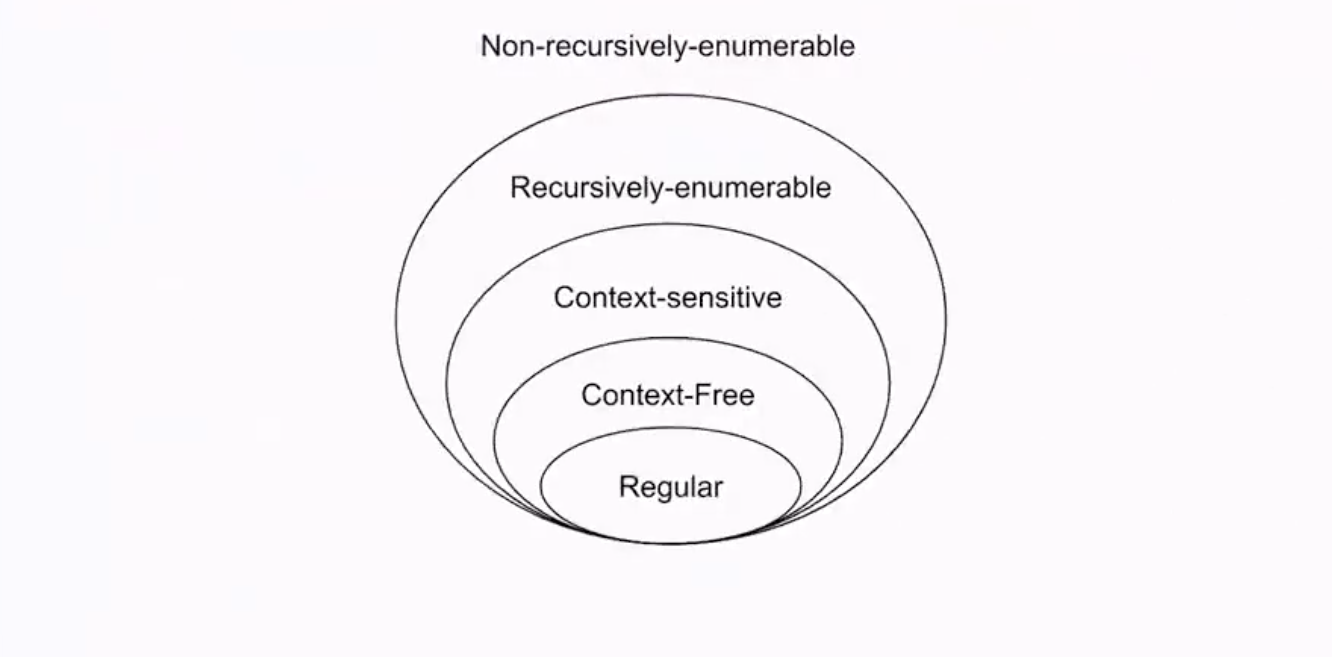
\includegraphics[width=\textwidth]{lecture1/images/chomsky-hierarchy.png}
\end{itemize}

\subsection{Exponentiation, Kleene Star, etc.}
\begin{itemize}
    \item For a language $L \subseteq \sum^{\ast}$ and $n \in \mathbb{N}$, define $L^n$ inductively as follows:
        \begin{itemize}
            \item $L^n = \{ \epsilon \}$ if $n = 0$
            \item $L^n = L \cdot L^{n - 1}$ if $n > 0$
        \end{itemize}
    \item Define $L^{\ast} = \bigcup_{n \geq 0} L^n$, and $L^+ = \bigcup_{n > 0} L^n$
\end{itemize}
